\documentclass{beamer}
\usetheme[shownavsym]{AAUsimple}
\usefonttheme{structurebold}
%%%%%%%%%%%%%%%%%%%%%%%%%%%%%%%%%%
\usepackage[utf8]{inputenc}
\usepackage[dutch]{babel}
\usepackage[T1]{fontenc}
\usepackage{tikz}
\usepackage{hyperref}
\usepackage{lmodern}
\usepackage{microtype}
%%%%%%%%%%%%%%%%%%%%%%%%%%%%%%%%%%
% Gekleurde hyperlinks
\newcommand{\chref}[2]{%
	\href{#1}{{\usebeamercolor[bg]{AAUsidebar}#2}}%
}
\title[TedTalk]{Hart- en vaatziekten \& preventie} 
\date{\today}

\author[Edon Namani, et. al]
{%
	Edon Namani\\
    Anaïs van Haaren
}
\institute[%
	Faculteit Gezondheidswetenschappen\\
	Rijksuniversiteit Groningen\\
	Nederland
]
{%
	Faculteit Gezondheidswetenschappen\\
	Rijksuniversiteit Groningen\\
	Nederland

}

\pgfdeclareimage[height=1.5cm]{titlepagelogo}{AAUgraphics/semper_invicta.pdf}
\titlegraphic{%
	\pgfuseimage{titlepagelogo}
}

\begin{document}
% Titel
{\aauwavesbg%
	\begin{frame}[plain,noframenumbering]
	\titlepage
\end{frame}}
%%%%%%%%%%%%%%%

\begin{frame}{Stress en hoe vaak het voorkomt}
    \begin{columns}
        \column{.4\textwidth}
        \includegraphics[width=\textwidth]{nieuwe-gevallen-van-overspannenheid-2017.pdf}
        \column{.6\textwidth}
    \begin{block}{Bijna 145.000 nieuwe patiënten met overspannenheid in 2017}
        In 2017 kregen naar schatting 144.500 nieuwe patiënten de diagnose neurasthenie/surmenage (overspannenheid) bij de huisarts: 48.500 mannen en 96.000 vrouwen. Dit komt overeen met 5,7 nieuwe patiënten per 1.000 mannen en 11,1 per 1.000 vrouwen (Nivel Zorgregistraties eerste lijn).
    \end{block}
\end{columns}
\end{frame}

\begin{frame}{Risicofactoren}{Hart- en vaatziekten}
    \begin{columns}
        \column{.5\textwidth}
    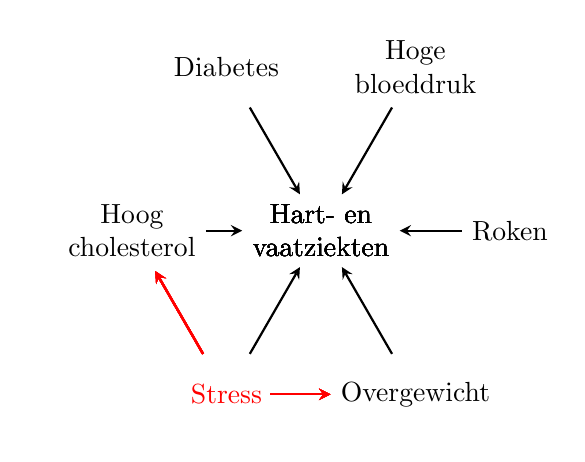
\begin{tikzpicture}[thick,>=stealth,->]
        \foreach[count=\x] \d/\f in {0/Roken,60/Hoge\\bloeddruk,120/Diabetes,180/Hoog\\cholesterol,240/\color{red}{Stress},300/Overgewicht}{
            \node[minimum size=1cm,align=center] (n\x) at (\d:2.4) {\f};
            \node[align=center] (H) at (0,0) {Hart- en \\ vaatziekten};
            \draw (n\x) -- (H);
            \node[minimum size=1cm] (d1) at (240:2.4) {\phantom{stress}};
            \node[minimum size=1cm] (d2) at (180:2.4) {\phantom{Hoog\\cholesterol}};
            \node[minimum size=1cm] (d3) at (300:2.4) {\phantom{Overgewicht}};
            \draw[color=red] (d1) -- (d2);
            \draw[color=red] (d1) -- (d3);
        }
    \end{tikzpicture}
    \column{.5\textwidth}
%    \begin{enumerate}
%        \item Roken
%        \item Hoge bloeddruk
%        \item Diabetes
%        \item Hoog cholesterol
%        \item Stress
%        \item Overgewicht
%    \end{enumerate}
\end{columns}
\end{frame}
\begin{frame}{Onderzoek}
    \begin{block}{Titel van het artikel}
        Effects of Exercise and Stress Management Training on Markers of Cardiovascular Risk in Patients with Ischemic Heart Disease\\
        A Randomized Control Trial
    \end{block}
\end{frame}
\begin{frame}{Onderzoek}{Conclusie}
    \includegraphics[width=.65\textwidth]{patienttree.pdf}
\end{frame}
%%%%%%%%%%%%%%%
\begin{frame}{Quote}{Levensfilosofie}
    \begin{block}{Lucius Annaeus Seneca}
    \begin{quote}
        A gem cannot be polished without friction, nor a man perfected without trials
    \end{quote}
\end{block}
\end{frame}

{\aauwavesbg
\begin{frame}[plain,noframenumbering]
	\finalpage{Bedankt voor het aandachtig luisteren!}
\end{frame}}
\end{document}
